\section {Formularea problemei}

În ora'se precum Bucure'sti, majoritatea blocurilor au fost contruite înainte de anul 1990 'si prin urmare interfoanele lor se bazează pe \acrshort{pots}. Trăind în era digitală, utilizatorul ideal î'si dore'ste augmentarea functionalitatilor sistemului existent, pentru a nu trebui să î'si convingă to'ti vecinii să învestească în modernizarea sistemului de acces. Pentru a putea adresa cât mai mul'ti utilizatori, solu'tia acestei probleme trebuie să fie agnostică de smartphoneul 'si interfonul existent al utilizatorului, dar să ofere integrări cu alte solu'tii de tip "Smart Home".

În func'tie de perioada instalării, sistemele să împart în două categorii: analogice 'si digitale. Posturile de interfon analogice sunt legate la o unitate de comandă care decodează semnale \acrfull{dtmf}, generează un semnal sinusoidal cu frecven'tă de 20Hz 'si amplitudinea de 60-90V pentru sonerie, apoi realizează conexiunile necesare dintre postul de afara 'si cel al apartamentului căutat. Sistemele digitale folosesc o magistrală comună de comunica'tii, fiind adresate conform unei scheme prestabilite - fiecare terminal este programat cu o adresă, însă pentru acest procedeu este nevoie de o cheie asociată unită'tii de comandă.

Din motive istorice, unitatea centrală \acrshort{pots} generează semnalul sinusoidal 'si poartă suficient curent pentru a putea alimenta clopotul apărut în prima genera'tie de telefoane. Prin urmare, sistemele digitale sunt considerate mai eficiente 'si mai sigure, dar 'si mai greu de integrat, datorită implicării unei persoane autorizate care să programeze întregul sistem.

Această lucrare vă analiza solu'tii digitale, însă sistemul final vă fi implementat pe un terminal analog. A'sadar, trebuie să în'telegem în primul rând mecanismul de adresare 'si cum este el interpretat de centrală. După cum insinuează numele, \acrshort{dtmf} presupune generarea a două tonuri de frecevente diferite în acela'si timp, conform liniei 'si coloanei tastei apăsate. Acest semnal vă fi intrepretat de decodorul de semnal al centralei cu ajutorul unor filtre de tip notch spre a se realiza conexiunile necesare. 

\begin{table}[ht!]
\begin{tabular}{c||c|c|c}
 & 1209Hz & 1336Hz & 1477Hz \\
\hline
\hline
697Hz & 1 & 2 & 3 \\
\hline
770Hz & 4 & 5 & 6 \\
\hline
852Hz & 7 & 8 & 9 \\
\hline
941Hz & * & 0 & \# \\
\end{tabular}
\centering
\caption{Tabel frecven'te \acrshort{dtmf}}
\label{tab:dtmf}
\end{table}

Sistemul descris până acum poate adresa $12-1=11$ posturi diferite (centrala este considerată 'si ea post 'si are un slot rezervat). Pentru a adresa mai multe posturi, unitatea de comandă trebuie să includă 'si un circuit logic secven'tial pentru a re'tine starea ultimelor taste apăsate. Astfel, ajungem la un număr satisfăcător de adrese pentru aplica'tia interfonului. 

Un exemplu de analiza spectrală a unui astfel de semnal:

\begin{figure}[h!]
  \centering
  \fbox {
    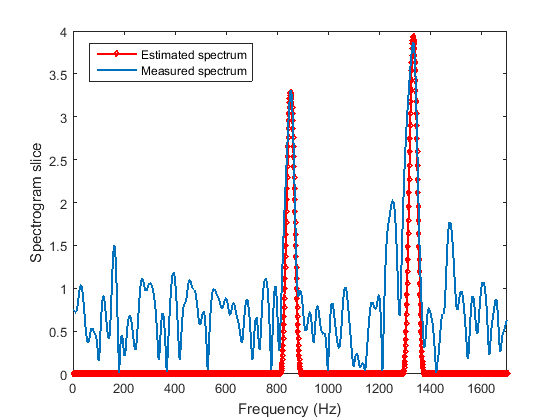
\includegraphics[width=\singlefigure]{02/04_spectru_dtmf.png}  
  }
  \caption{Spectrogramă tasta "8" \cite{AunsriNattapol2016}}
\end{figure}

Se pot distinge grafic două frecven'te predominante: 852Hz 'si 1336Hz - cobinatia corespunaztoare tastei "8".

\section {Studiu asupra realizărilor similare din domeniu}


\subsection {Videx UK}

Interfoanele \acrshort{gsm} de la Videx sunt conectate la re'teaua mobilă de telefonie 'si permit operarea unei por'ti prin intermediul unui releu. Ele necesită doar o sursă de curent externă, o antenă 'si o cartelă \acrfull{sim} pentru a opera.

\begin{figure}[h!]
  \centering
  \fbox {
    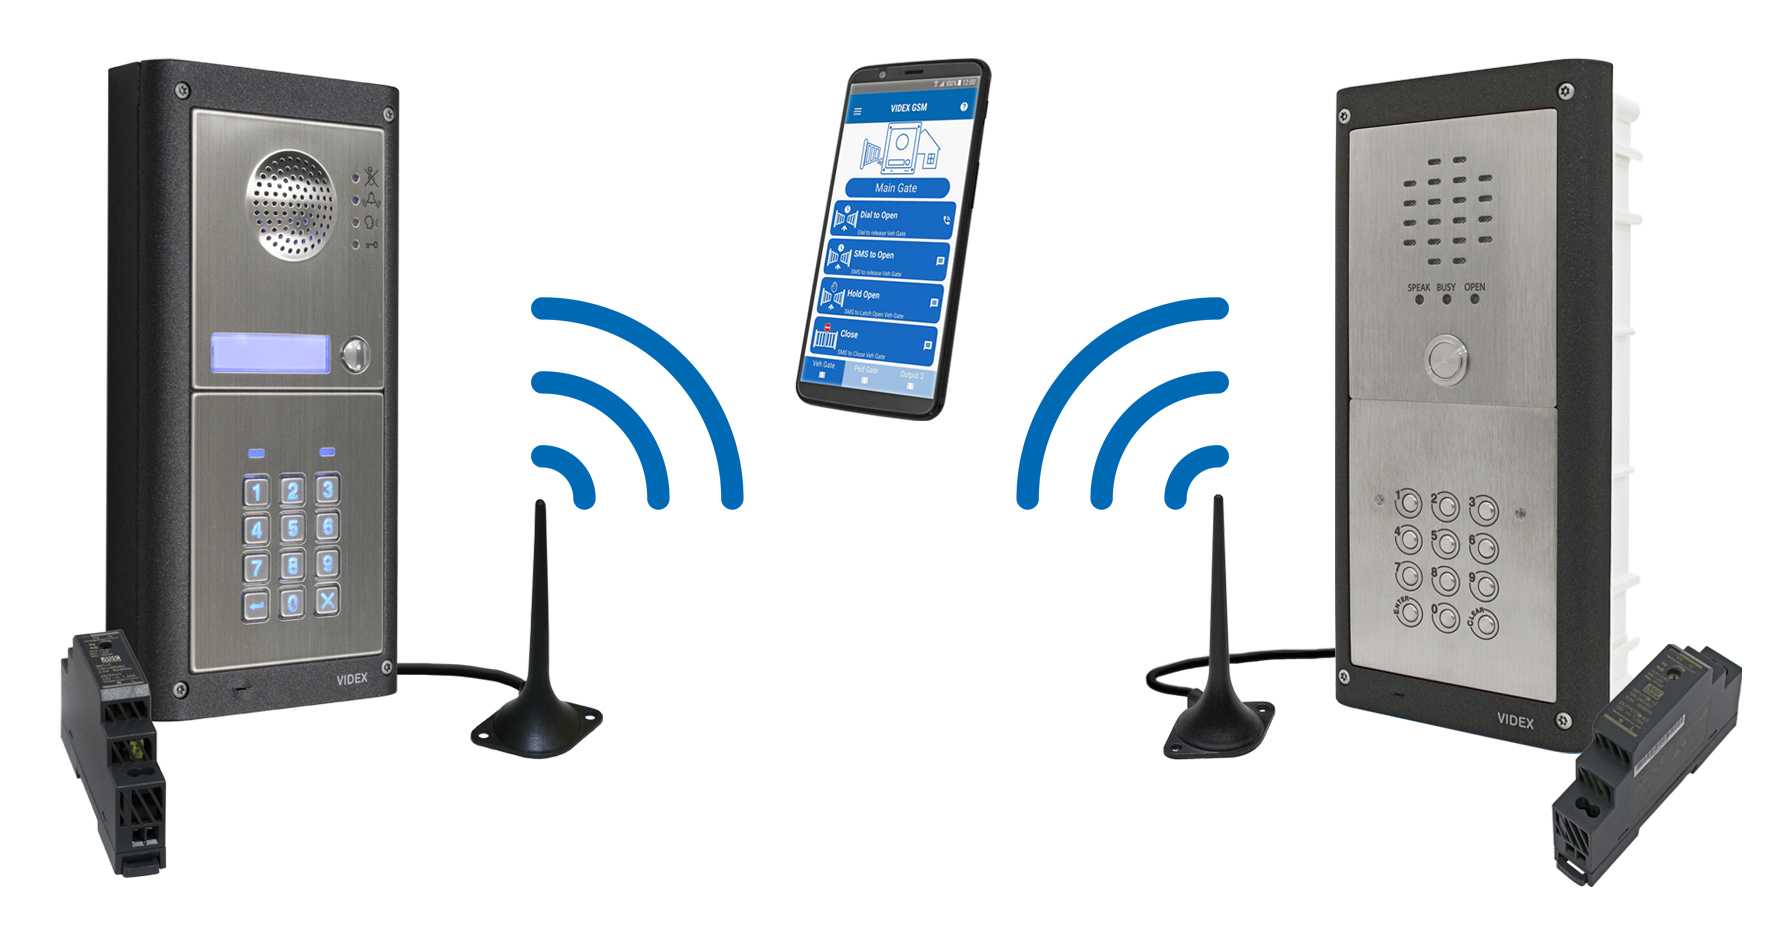
\includegraphics[width=\singlephoto]{02/01_gsm_system.jpg}  
  }
  \caption{Sistem interfon Videx GSM \cite{VidexUk}}
\end{figure}

Printre func'tionalită'tile principale se numără:
\begin{itemize}
  \item Poate include un cititor de carduri \acrshort{rfid} 'si cheie
  \item Versiune rezistentă la vandalism
  \item Până la 4 numere de telefon per apartament, pentru redundantă. În cazul în care primul număr nu se poate apela sau nu răspunde, se vă încercă următorul număr programat
  \item Oferă aplica'tie Android 'si iOS pentru programat unitatea
\end{itemize}

Dezavantaje:

\begin{itemize}
  \item Nu oferă integrare cu servicii din re'teaua \acrshort{iot}
\end{itemize}

\subsection {Google Nest x Yale Lock}

\begin{figure}[h!]
  \centering
  \fbox {
    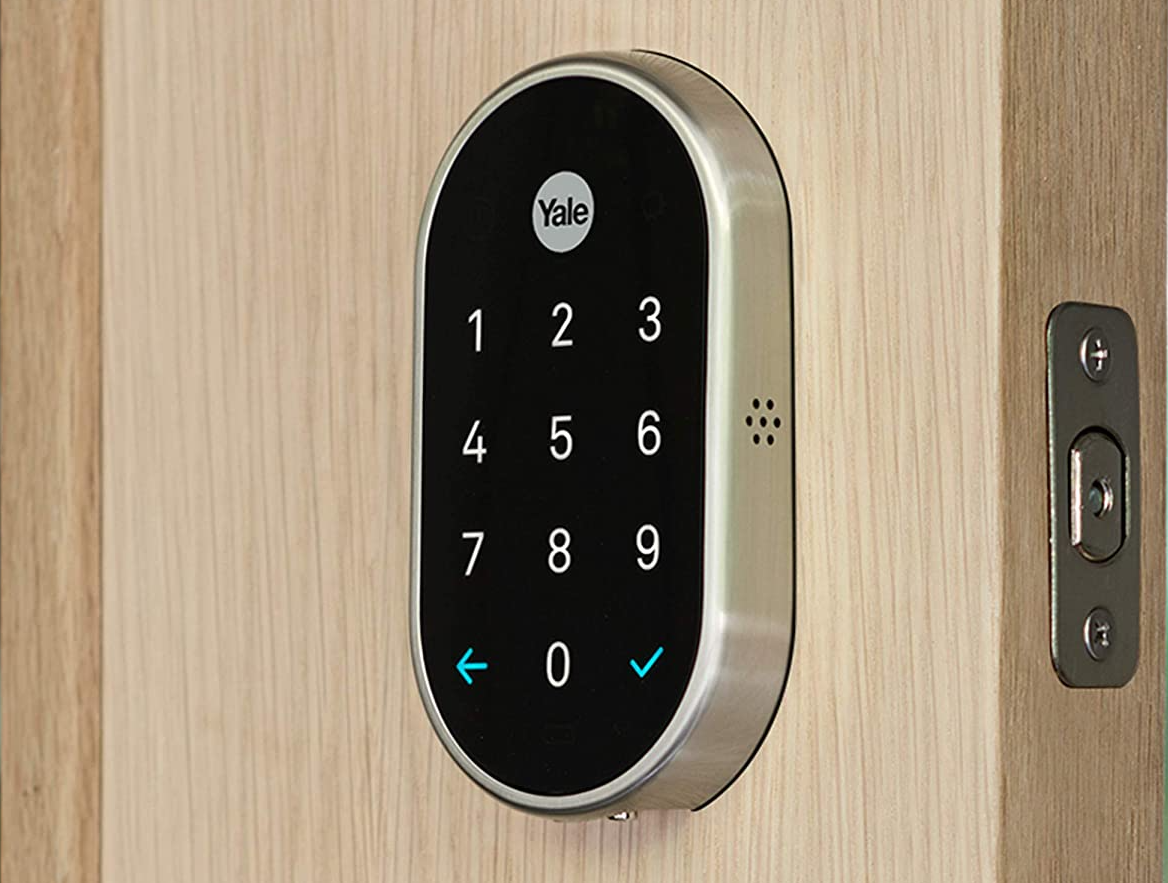
\includegraphics[width=\singlephoto]{02/02_iot_system.png}  
  }
  \caption{Next x Yale Lock \cite{YaleLock}}
\end{figure}

Avantaje:
\begin{itemize}
  \item Permite accesul prin intermediul unui PIN ales de utilizator
  \item Oferă alerte când cineva închide sau deschide u'sa
  \item Oferă integrare cu Google Home 'si Nest Home
\end{itemize}

Dezavantaje:
\begin{itemize}
  \item Are nevoie de 4 baterii tip AA pentru a func'tionă
  \item Nu are acces cu cheie sau cartelă
  \item Nu are versiune rezistentă
\end{itemize}


\subsection {Level Lock - Touch Edition}

Level Lock este o încuietoare inteligentă de tip zăvor. Are un design minimalist 'si ascunde partea electronică în interiorul u'sii pentru mai multă securitate.

\begin{figure}[h!]
  \centering
  \fbox {
    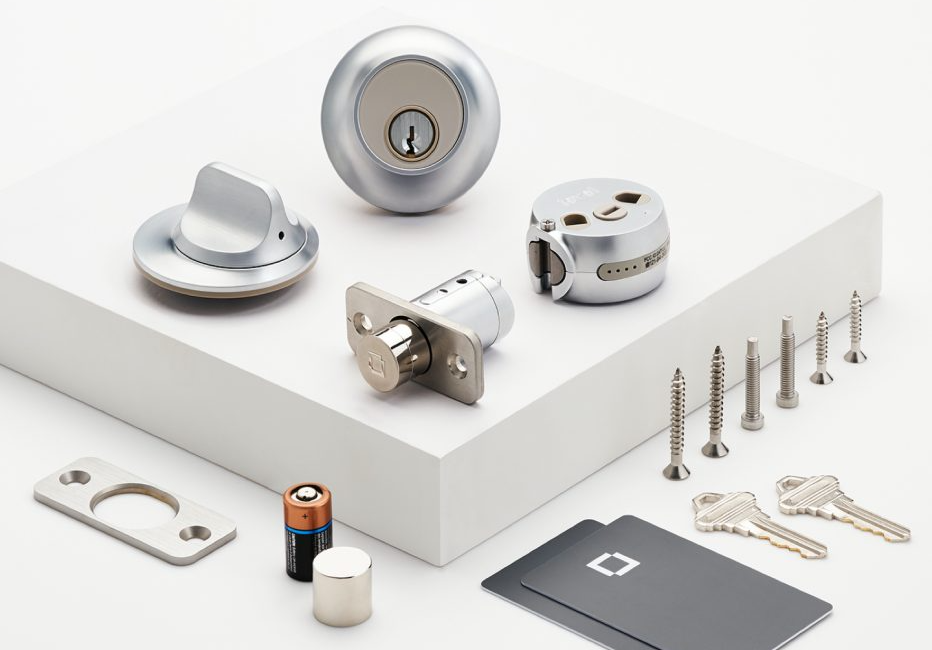
\includegraphics[width=\singlephoto]{02/03_iot_system.jpg}  
  }
  \caption{Level Lock \cite{LevelLock}}
\end{figure}

Avantaje:
\begin{itemize}
  \item Multiple modalită'ti de acces, printre care: amprentă, PIN
  \item Oferă alerte când cineva închide sau deschide u'sa
  \item Oferă integrare cu Google Home 'si Nest Home
\end{itemize}

\subsection {Compara'tii}

Produsele de mai sus adresează probleme u'sor diferite, dar încearcă să ofere func'tionalită'ti similare. Sistemul oferit de Videx Security prezinta un design rezistent, dar familiar tuturor utilizatorilor 'si este destinat clădirilor cu mai mul'ti locatari. În contrast, cele două încuietori inteligente oferă o integrare avansată în re'teaua \acrshort{iot} 'si multiple căi de acces, dar sunt destinate unei singure locuin'te.

Încuietoarea de la Yale prezintă cea mai inovativa abordare a acestul design prin decizia deliberată de a nu oferi posibilitatea de acces cu cheie. Astfel, simplifică partea mecanică eliminând singura cale de acces din exterior către mecanismul încuietorii.

Produsul celor de la Videx Security se bazează pe o tehnologie utilizată la scară largă 'si prin urmare beneficiază de robuste'tea unui sistem matur. Spre deosebire de celelalte două produse analizate, solu'tia celor de la Videx Security este agnostică de sistemul de operare al telefonului mobil, având nevoie doar de o conexiune \acrshort{gsm}.

Din lipsa unor standarde în domeniu, dispozitivele noi suferă de alte tipuri de probleme 'si vulnerabilită'ti, după un studiu realizat de cercetătorii de la Bitdefender. Majoritatea sunt în faza ini'tială de setare, oferind protocoale de securitate învechite sau omitandu-le complet. Este men'tionat 'si un dispozitiv care expune un port Telnet, un protocol învechit 'si u'sor de exploatat, fără posibilitatea de a fi dezactivat \cite{Bitdefender2016IoT}.

\section {Stabilirea cerin'telor func'tionale 'si nefunc'tionale ale sistemului}

Cerin'tele func'tionale ale acestui sistem vor fi împăr'tite conform tabelului următor, ele fiind detaliate mai jos.

\begin{table}[ht!]
\begin{tabular}{l|l}
\hline
Cerin'te func'tionale (F) & Cerin'te nefunc'tionale (NF) \\
\hline
\hline
\textbf{F1.} Controlul accesului în apartament & \textbf{NF1.} Func'tie răspuns automat \\
\hline
\textbf{F2.} Expunerea unui serviciu REST & \textbf{NF2.} Control granular asupra datelor \\
\hline
\textbf{F3.} Dezvoltare client Android & \textbf{NF3.} Expunerea unui flux duplex VoIP \\
\hline
\textbf{F4.} Criptarea informa'tiilor transmise & \\
\hline
\textbf{F5.} Managementul accesului la sistem & \\
\hline
\end{tabular}
\centering
\caption{Tabel stabilire cerin'te}
\label{tab:funcnefunc}
\end{table}

\subsection{(F1) Controlul accesului în apartament}

Scopul principal al acestui sistem este de a oferi sau nu acces într-o incintă, prin urmare consider aceasta cea mai importantă cerin'tă func'tională.

\subsection{(F2) Expunerea unui serviciu REST pentru interfa'tarea cu alte sisteme}

Expunerea 'si abstractizarea terminalului \acrshort{pots} este realizată printr-un set de servicii \acrfull{rest} care controlează starea sa. Acest lucru ne permite interfa'tarea cu aplica'tia mobilă, interfa'ta de administrare web 'si alte servicii precum Google Home/Google Assistant/Apple HomeKit.

\subsection{(F3) Dezvoltarea unui client mobil Android}

Principalul client care va interac'tiona cu serviciile \acrshort{rest} va fi aplica'tia mobilă ce vă avea rolul de a notifica userul în eventualitatea declan'sării soneriei interfonul 'si de a controla starea sistemului.

\subsection{(F4) Criptarea comunica'tiilor cu serviciile web}

Având în vedere nivelul de acces pe care l-ar oferi o exploatare a unei vulnerabilitati al acestei solu'tii, comunica'tiile între server 'si clien'ti trebuie realizate printr-un canal criptat de tip \acrfull{ssl}. Credentialele u'serului 'si ulterior tokenul de acces trebuie trimise doar după verificarea autenticită'tii serverului 'si a pachetelor trimise.

\subsection{(F5) Oferirea 'si revocarea accesului la sistem}

Dorim de exemplu să oferim acces necondi'tionat unui prieten apropiat pentru a intra în bloc fară a mai suna la interfon. De asemenea ar trebui să putem realiza 'si inversul acestei opera'tii.


\subsection{(NF1) Implementarea unei func'tii pentru răspuns automat}

Această func'tie vă permite utilizatorului să stabilească o perioadă de timp pentru care sistemul vă oferi accesul necondi'tionat.

\subsection{(NF2) Control granular asupra datelor stocate}

Arhitectura aplica'tiei necesită interac'tiunea cu o bază de date, care poate fi 'tinută în cloud, pentru convenabilitate sau local.
Folosind tehnologii de containerizare precum Docker, putem stoca baza de date local, informa'tiile fiind stocate într-un mediu controlat.

\subsection{(NF3) Expunerea unui flux duplex audio prin tehnologia VoIP}

Pasul final în dezvoltarea acestui sistem ar fi interfa'tarea cu un \acrfull{adc} 'si un \acrfull{dac} 'si expunerea streamurilor de date prin \acrfull{voip}

